\input{../../../.preambles/02-lab_work}
\newgeometry{top=1.5cm, bottom=1.5cm, left=1cm, right=1cm}
\begin{document}
    \begin{table}[h!]
        \center
        \begin{tabular}{|C{.5}|C{.2}|C{.25}|}
            \hline
            \multicolumn{1}{|c|}{\multirow{4}{*}{Лабораторная работа № 1}} &
            Студент, группа & {{ student }}, Ф-369 \\ \cline{2-3}
            & Дата выполнения & 06.03.2013 \\ \cline{2-3}
            & Подпись &  \\ \cline{2-3}
            & Дата отчёта & \\ \cline{2-3}
            Изучение процесса радиоактивного распада & Оценка &  \\ \cline{2-3}
            & Подпись &  \\ \hline
        \end{tabular}
    \end{table}

    \emph{Цель работы:} изучение основного закона радиоактивного распада
    с помощью компьютерного моделирования.

    \subsection{Селен (Se)}
    \vspace*{-1em}

    \begin{table}[ht]
        \center
        \caption{Результаты эксперимента для селена}
        \begin{tabular}{|*{15}{C{.045}|}} \hline
            \multicolumn{3}{|c|}{Атомная масса} &
            \multicolumn{4}{c|}{Период полураспада} &
            \multicolumn{4}{c|}{Постоянная распада} &
            \multicolumn{4}{c|}{Количество полупериодов} \\
            \hline
            %-------------------------------------------------------------------
            \multicolumn{3}{|c|}{73} & \multicolumn{4}{c|}{7,1 часа} &
            \multicolumn{4}{c|}{0,09763} & \multicolumn{4}{c|}{7} \\ \hline
            %-------------------------------------------------------------------
            \( t \),~час. & 0 & 3,823 & 7,646 & 11,469 & 15,292 & 19,115 &
            22,938 & 26,762 & 30,585 & 34,408 & 38,231 & 42,054 & 45,877 &
            49,700 \\ \hline
            %-------------------------------------------------------------------
            \multirow{5}{*}{\(N_\emph{отн}\)}
            & 1,007 & 0,680 & 0,457 & 0,353 & 0,195 & 0,116 & 0,114 & 0,070 &
            0,044 & 0,038 & 0,021 & 0,018 & 0,012 & 0,008 \\ \cline{2-15}
            & 0,933 & 0,704 & 0,519 & 0,327 & 0,241 & 0,158 & 0,095 & 0,068 &
            0,045 & 0,035 & 0,023 & 0,016 & 0,012 & 0,007 \\ \cline{2-15}
            & 1,106 & 0,555 & 0,498 & 0,388 & 0,248 & 0,158 & 0,087 & 0,085 &
            0,057 & 0,030 & 0,026 & 0,019 & 0,011 & 0,007 \\ \cline{2-15}
            & 0,976 & 0,744 & 0,459 & 0,276 & 0,235 & 0,179 & 0,105 & 0,078 &
            0,049 & 0,044 & 0,023 & 0,015 & 0,010 & 0,007 \\ \cline{2-15}
            & 0,988 & 0,868 & 0,497 & 0,302 & 0,199 & 0,166 & 0,125 & 0,059 &
            0,056 & 0,034 & 0,028 & 0,014 & 0,010 & 0,007 \\ \hline
            %-------------------------------------------------------------------
            \( \midnum{N} \) & 1,002 & 0,710 & 0,486 & 0,329 & 0,224 & 0,155 &
            0,105 & 0,072 & 0,050 & 0,036 & 0,024 & 0,016 & 0,011 & 0,007
            \\ \hline
            %-------------------------------------------------------------------
            \( \sigma \) & 0,064 & 0,113 & 0,027 & 0,044 & 0,025 & 0,024 &
            0,015 & 0,010 & 0,006 & 0,005 & 0,003 & 0,002 & 0,001 & 0,001 \\
            \hline
        \end{tabular}
    \end{table}
    
    \begin{figure}[h!]
        \center
        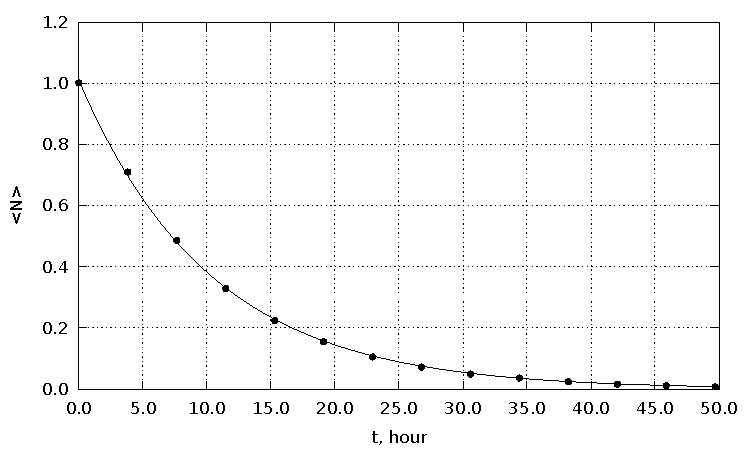
\includegraphics[width=.47\textwidth]{Se_N} \hfill
        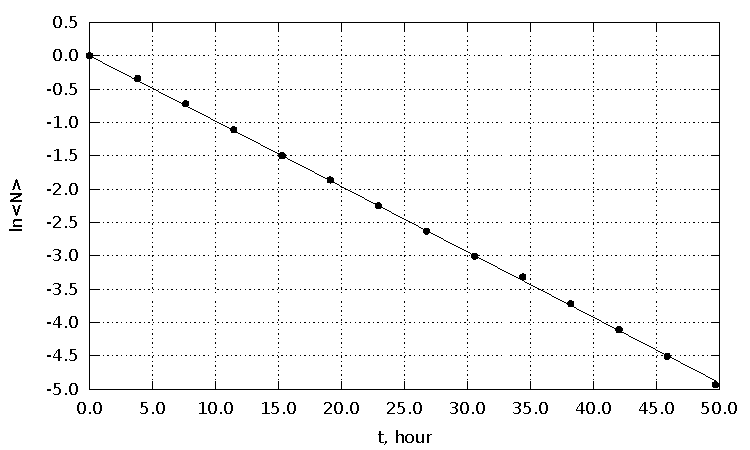
\includegraphics[width=.47\textwidth]{Se_lnN}
        \parbox{.47\textwidth}{\caption{Зависимость \( \midnum{N} \) от времени}} \hfill
        \parbox{.47\textwidth}{\caption{Зависимость \( \ln \midnum{N} \) от времени}}
    \end{figure}

    Экспериментальное значение постоянной распада для селена:
    \( \lambda_\mathrm{Se} = 0,\!09804 \).

    \newpage

    \subsection{Иттрий (Y)}
    \vspace*{-1em}

    \begin{table}[ht]
        \center
        \caption{Результаты эксперимента для иттрия}
        \begin{tabular}{|*{15}{C{.045}|}} \hline
            \multicolumn{3}{|c|}{Атомная масса} &
            \multicolumn{4}{c|}{Период полураспада} &
            \multicolumn{4}{c|}{Постоянная распада} &
            \multicolumn{4}{c|}{Количество полупериодов} \\
            \hline
            %-------------------------------------------------------------------
            \multicolumn{3}{|c|}{92} & \multicolumn{4}{c|}{3,5 часа} &
            \multicolumn{4}{c|}{0,19804} & \multicolumn{4}{c|}{7} \\ \hline
            %-------------------------------------------------------------------
            \( t \),~час. & 0 & 1,885 & 3,769 & 5,654 & 7,538 & 9,423 & 11,308 &
            13,192 & 15,077 & 16,962 & 18,846 & 20,731 & 22,615 & 24,500 \\
            \hline
            %-------------------------------------------------------------------
            \multirow{5}{*}{\(N_\emph{отн}\)}
            & 1,268 & 0,668 & 0,513 & 0,313 & 0,186 & 0,158 & 0,099 & 0,066 &
            0,053 & 0,032 & 0,025 & 0,014 & 0,010 & 0,007 \\ \cline{2-15}
            & 1,111 & 0,699 & 0,465 & 0,311 & 0,228 & 0,163 & 0,108 & 0,080 &
            0,056 & 0,035 & 0,021 & 0,014 & 0,012 & 0,008 \\ \cline{2-15}
            & 1,023 & 0,665 & 0,398 & 0,348 & 0,193 & 0,157 & 0,108 & 0,075 &
            0,053 & 0,037 & 0,021 & 0,014 & 0,012 & 0,008 \\ \cline{2-15}
            & 0,986 & 0,703 & 0,461 & 0,356 & 0,216 & 0,166 & 0,109 & 0,077 &
            0,046 & 0,036 & 0,024 & 0,016 & 0,012 & 0,008 \\ \cline{2-15}
            & 1,037 & 0,615 & 0,420 & 0,348 & 0,221 & 0,166 & 0,106 & 0,079 &
            0,045 & 0,049 & 0,027 & 0,020 & 0,012 & 0,009 \\ \hline
            %-------------------------------------------------------------------
            \( \midnum{N} \) & 1,085 & 0,670 & 0,451 & 0,335 & 0,209 & 0,162 &
            0,106 & 0,075 & 0,051 & 0,036 & 0,024 & 0,016 & 0,012 & 0,008 \\
            \hline
            %-------------------------------------------------------------------
            \( \sigma \) & 0,112 & 0,035 & 0,044 & 0,021 & 0,018 & 0,004 &
            0,004 & 0,006 & 0,005 & 0,003 & 0,003 & 0,003 & 0,001 & 0,001 \\
            \hline
        \end{tabular}
    \end{table}
    
    \begin{figure}[h!]
        \center
        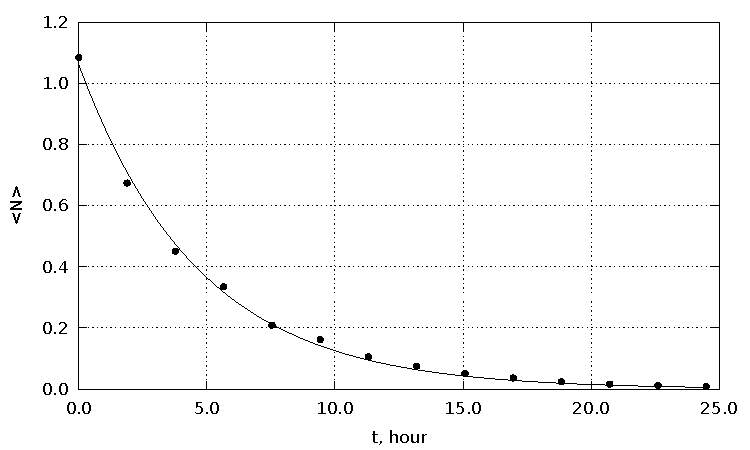
\includegraphics[width=.47\textwidth]{Y_N} \hfill
        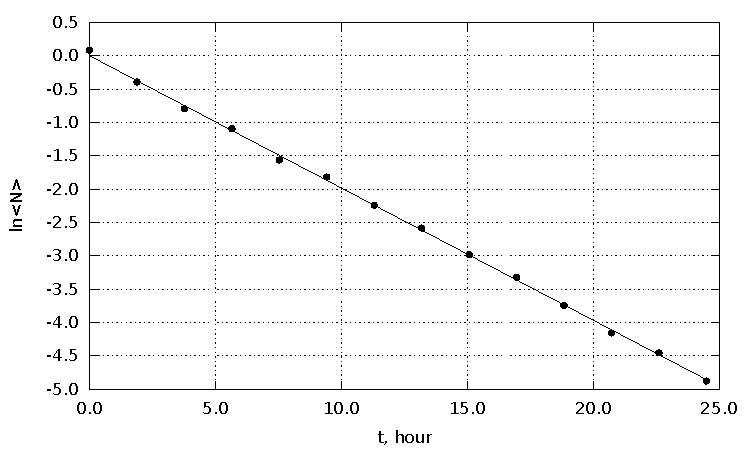
\includegraphics[width=.47\textwidth]{Y_lnN}
        \parbox{.47\textwidth}{\caption{Зависимость \( \midnum{N} \) от времени}} \hfill
        \parbox{.47\textwidth}{\caption{Зависимость \( \ln \midnum{N} \) от времени}}
    \end{figure}

    Экспериментальное значение постоянной распада для иттрия:
    \( \lambda_\mathrm{Y} = 0,\!19833 \).

    \newpage

    \subsection{Неон (Ne)}
    \vspace*{-1em}

    \begin{table}[ht]
        \center
        \caption{Результаты эксперимента для неона}
        \begin{tabular}{|*{15}{C{.045}|}} \hline
            \multicolumn{3}{|c|}{Атомная масса} &
            \multicolumn{4}{c|}{Период полураспада} &
            \multicolumn{4}{c|}{Постоянная распада} &
            \multicolumn{4}{c|}{Количество полупериодов} \\
            \hline
            %-------------------------------------------------------------------
            \multicolumn{3}{|c|}{24} & \multicolumn{4}{c|}{3,38 минуты} &
            \multicolumn{4}{c|}{0,20507} & \multicolumn{4}{c|}{7} \\ \hline
            %-------------------------------------------------------------------
            \( t \),~мин. & 0 & 1,82 & 3,64 & 5,46 & 7,28 & 9,10 & 10,92 &
            12,74 & 14,56 & 16,38 & 18,20 & 20,02 & 21,84 & 23,66 \\
            \hline
            %-------------------------------------------------------------------
            \multirow{5}{*}{\(N_\emph{отн}\)}
            & 1,144 & 0,718 & 0,481 & 0,327 & 0,213 & 0,164 & 0,114 & 0,061 &
            0,049 & 0,036 & 0,027 & 0,017 & 0,014 & 0,008 \\ \cline{2-15}
            & 1,078 & 0,605 & 0,406 & 0,343 & 0,220 & 0,139 & 0,097 & 0,073 &
            0,056 & 0,039 & 0,024 & 0,016 & 0,011 & 0,007 \\ \cline{2-15}
            & 1,064 & 0,652 & 0,470 & 0,328 & 0,233 & 0,136 & 0,127 & 0,077 &
            0,046 & 0,037 & 0,026 & 0,017 & 0,011 & 0,009 \\ \cline{2-15}
            & 1,024 & 0,601 & 0,455 & 0,382 & 0,242 & 0,143 & 0,102 & 0,079 &
            0,057 & 0,041 & 0,025 & 0,022 & 0,010 & 0,009 \\ \cline{2-15}
            & 0,766 & 0,636 & 0,460 & 0,322 & 0,250 & 0,150 & 0,111 & 0,077 &
            0,062 & 0,036 & 0,023 & 0,013 & 0,011 & 0,007 \\ \hline
            %-------------------------------------------------------------------
            \( \midnum{N} \) & 1,015 & 0,642 & 0,454 & 0,340 & 0,232 & 0,146 &
            0,110 & 0,073 & 0,054 & 0,038 & 0,025 & 0,017 & 0,011 & 0,008 \\
            \hline
            %-------------------------------------------------------------------
            \( \sigma \) & 0,146 & 0,047 & 0,029 & 0,025 & 0,015 & 0,011 &
            0,012 & 0,007 & 0,006 & 0,002 & 0,002 & 0,003 & 0,002 & 0,001 \\
            \hline
        \end{tabular}
    \end{table}
    
    \begin{figure}[h!]
        \center
        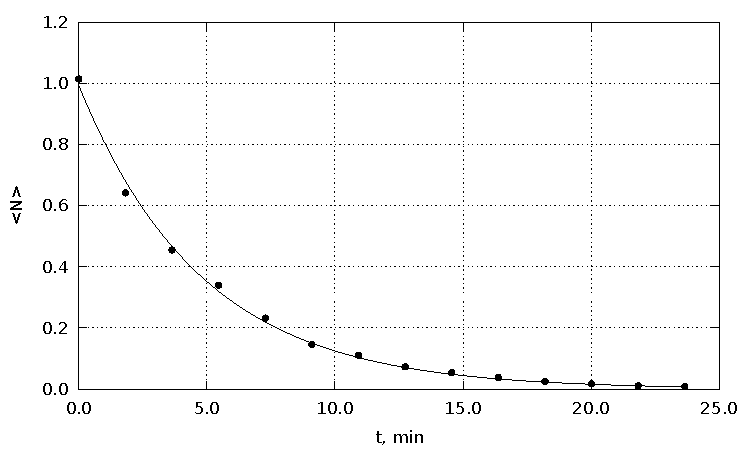
\includegraphics[width=.47\textwidth]{Ne_N} \hfill
        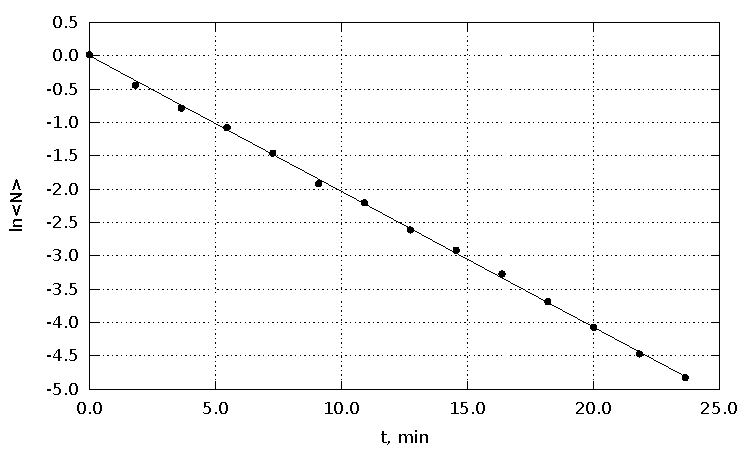
\includegraphics[width=.47\textwidth]{Ne_lnN}
        \parbox{.47\textwidth}{\caption{Зависимость \( \midnum{N} \) от времени}} \hfill
        \parbox{.47\textwidth}{\caption{Зависимость \( \ln \midnum{N} \) от времени}}
    \end{figure}

    Экспериментальное значение постоянной распада для неона:
    \( \lambda_\mathrm{Ne} = 0,\!20342 \).
    
    \vspace*{2em}
    \emph{Вывод:} провел опыты, моделирующие радиоактивные распады, в которых
    измерялось относительное количество частиц с течением времени. После по
    полученным данным построил графики зависимости \( \ln \midnum{N} \) от
    времени, из которых были получены экспериментальные значения постоянных
    распада \( \lambda \), практически не отличающихся от теоретических.
\end{document}
